\documentclass[brudnopis]{xmgr}
%\documentclass[xodstep]{xmgr}

%\defaultfontfeatures{Scale=MatchLowercase}
%\setmainfont[Numbers=OldStyle,Ligatures=TeX]{Minion Pro}
%\setsansfont[Numbers=OldStyle,Ligatures=TeX]{Myriad Pro}
% for fontspec version < 2.0
\setmainfont[Numbers=OldStyle,Mapping=tex-text]{Minion Pro}
\setsansfont[Numbers=OldStyle,Mapping=tex-text]{Myriad Pro}
%\setmonofont[Scale=0.75]{Monaco}

% Opcjonalnie identyfikator dokumentu 
% drukowany tylko z włączoną opcją 'brudnopis':
\wersja   {}

\author   {Dorian Sawa}
\nralbumu {186\,445}
\email    {dsawa@sigma.ug.edu.pl}

\title    {System weryfikacji jakości kodu \newline w języku Scala}
\date     {2014}
\miejsce  {Gdańsk}

\opiekun  {dr Wiesław Pawłowski}

\usepackage{minted}
	\renewcommand\listingscaption{Przykład}
	
\makeatletter
\minted@define@extra{label}
\makeatother
	
\fvset{
	fontsize=\small
}

% dodatkowe polecenia
%\renewcommand{\filename}[1]{\texttt{#1}}

\begin{document}

\begin{abstract}
Scala to język wspierający paradygmaty programowania obiektowego i funkcyjnego. Rosnąca w ostatnim czasie popularność Scali przyczyniła się do powstania wielu narzędzi pozwalających na testowanie programów napisanych właśnie w tym języku. Niniejsza praca zgłębia temat wspomnianych narzędzi oraz ich wykorzystania jako podstawy systemu pozwalającego na automatyzację kontroli jakości kodu.
\end{abstract}
\keywords{Scala, 
 Play Framework, 
 Simple Build Tool,
 SBT,
 ScalaTest, 
 ScalaCheck,
 ScalaStyle}

% tytuł i spis treści
\maketitle
%
% wstęp
\introduction Scala jest nowoczesnym językiem programowania działającym na wirtualnej maszynie Javy. Od chwili opublikowania jest ona sukcesywnie rozwijana. Współcześnie wiele firm korzysta z systemów napisanych w Scali. Systemy takie, napisane dla celów wewnętrznych, czy też komercyjnych spełniają swoje zadania z sukcesami. Wśród firm korzystających z technologii Scali znaleźć można między innymi LinkedIn, Twitter czy Intel. Chociaż Scala jest językiem całkowicie zorientowanym obiektowo, to posiada on także wszystkie elementy jakie można oczekiwać od języka funkcyjnego.

Przy wielu zaletach jakie ze sobą niesie możliwość programowania w Scali, udział procentowy tego języka na tle konkurencji wciąż jest stosukowo nieduży. Oczywiście proporcjonalnie do takiego rozkładu wygląda również sytuacja programistów Scali na rynku pracy. Jednym z impulsów do zmiany tego faktu mogłaby być specjalna platforma pozwalająca przyspieszyć proces nauki Scali. Na tym zagadnieniu skupia się niniejsza praca.

Zaprojektowany i opisywany tu system powstał na bazie nowoczesnych technologii oraz najważniejszych narzędzi do testów jednostkowych. Podstawą systemu jest Play Framework. Pozwala on na szybkie napisanie aplikacji internetowej zarówno w Scali jak i w Javie. Społeczność powstała wokół tych dwóch języków doprowadziła do powstania ogromnej liczby bibliotek. Z powodzeniem mogą być one używane w aplikacji utworzonej przy użyciu Play Framework. 

Pośród bibliotek związanych z testowaniem kodu na szczególną uwagę zasługuje Scalatest oraz Scalacheck. Pierwsza z nich to biblioteka do przeprowadzania testów jednostkowych. Umożliwia ona między innymi pisanie testów w wielu różnych stylach. Decyzja o tym jak ostatecznie wyglądać będzie test zależy od preferencji użytkownika. Scalacheck jest zaś instrumentem służącym do testowania funkcji, metod poprzez automatyczne wprowadzanie różnych argumentów. 

Projektując system do weryfikacji kodu Scala zdecydowałem się skorzystać z nierelacyjnej bazy danych z wbudowanym mechanizmem do przechowywania plików - MongoDB. Interfejs użytkownika powstał zaś przy pomocy AngularJS, który w przyjemny dla programisty sposób  potrafi dynamicznie zmieniać zawartość strony HTML warunkując ją od akcji użytkownika mających wpływ na stan modeli aplikacji.

\medskip Na początku swojej pracy postaram się szerzej przedstawić ideę będącą iskrą do stworzenia tego systemu. Pokażę, że dla innych języków programowania już funkcjonują pewne mechanizmy edukacyjne. Kolejnym krokiem będzie prezentacja języka Scala. Opowiem o mechanizmie aktorów, kombinacji języka funkcyjnego i obiektowego oraz innych nowych rzeczach jakie ze sobą niesie. Każde ze wspominanych wcześniej narzędzi zostanie również szerzej przedstawione. Każde z nich wywarło wpływ na ostateczny kształt opisywanej aplikacji. Ustosunkuję się do wyboru tych narzędzi spośród innych. Między innymi dlaczego zdecydowałem się na użycie nierelacyjnego MongoDB. I czemu uznałem, że standardowa funkcjonalność AngularJS to było dla mnie za mało. Ostatecznie przybliżę także sposób działania systemu oraz w jaki sposób użyte zostało jeszcze jedno narzędzie - SBT. Bezpośrednio związane z weryfikacją kodu uczestników systemu. 

\chapter{Idea systemu}

Wykonując odpowiednie zapytanie przy użyciu narzędzia \textit{Google BigQuery} oraz danych z \textit{Github Archive} można w prosty sposób sprawdzić popularność języków programowania na platformie \textit{GitHub}. Ilość repozytoriów dla poszczególnych języków w roku 2013  przedstawia rysunek \ref{RYS.1}. 

\begin{figure}[!tbh]
\centering 
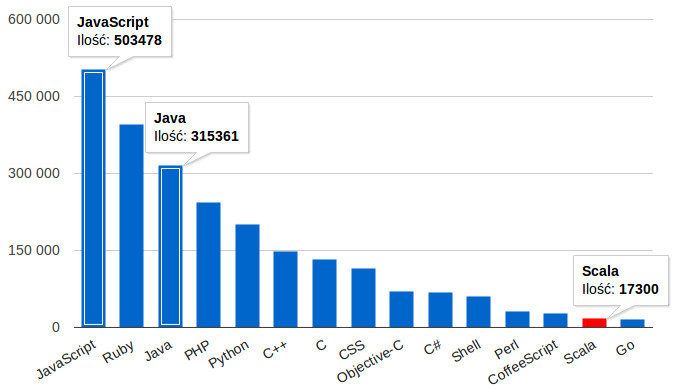
\includegraphics[width=.95\hsize]{fig/top_github_languages_2013}
\caption{Ilość repozytoriów dla poszczegónych języków na platformie GitHub w roku 2013 \label{RYS.1}}
\source{GitHub Archive (www.githubarchive.org)}
\end{figure}

Powyższy wykres przedstawia pierwszych 15 języków, wśród których Scala uplasowała się na miejscu 14. Różnica w liczbie repozytoriów między Scalą, a Javą będącą na trzecim miejscu jest znaczna. Nie ma wątpliwości, że Java swoją wysoką pozycje zawdzięcza wieloletniej obecności na rynku, a także wkładowi jaki do świata technologii informacyjnych wniosła maszyna wirtualna JVM. Na popularność JavaScript'u, czy Ruby'ego częściowo miało wpływ pojawienie się w ostatniej dekadzie narzędzi takich jak \textit{Ruby on Rails}, \textit{node.js}, \textit{AngularJS} i wielu innych. 

Jednak jak pokazuje przykład Ruby'ego i JavaScriptu, jednym z elementów wpływających na popularność jest aktywne środowisko programistów zgromadzonych wokół danego języka. Niejednokrotnie, taka grupa osób przekonana o zaletach swojego ulubionego języka jest w stanie wytworzyć alternatywne sposoby jego promocji. Potwierdzeniem tego może być zespół programistów zgromadzonych wokół platformy \textit{CodeSchool}\footnote{www.codeschool.com}. Opracowali oni szereg prostych kursów związanych głownie z JavaScript'em i Ruby'm w trakcie, których uczestnik rozwiązuje proste zadania programistyczne. 

Żadne z obecnych rozwiązań - szczególnie dla Scali - nie posiada jednak możliwości tworzenia własnych zadań dla zamkniętych grup uczestników. Wierzę, że system, który daje sposobność definiowania własnych kursów dla języka Scala może znacząco zwiększyć jej popularność. Implementacja takiego systemu w szkołach i uczelniach mogłaby przynieść również inne korzyści, jak na przykład wzrost zainteresowania programowaniem, czy podniesieniem umiejętności przyszłych programistów przy jednoczesnym zmniejszeniu nakładu pracy prowadzących zajęcia.

\section{Język Scala}

Pomysłodawcą i głównym twórcą Scali jest niemiecki profesor Martin Odersky. Nazwa języka ma na celu sugerować, że jest on skalowalny\footnote{ang: Scalable language}. Scala rośnie wraz z potrzebami jej użytkowników. Cały czas powstają kolejne narzędzia i biblioteki mające uprościć pracę z nią, czy też dodać do niej coś nowego. 

Scala łączy ze sobą paradygmat programowania obiektowego oraz funkcyjnego. Umożliwia wykorzystanie najlepszych cech tych dwóch podejść w projektowaniu nowych systemów. Sprawdzi się zatem doskonale zarówno podczas pisania małych jak i dużych projektów.

W przypadku tych pierwszych, programowanie funkcyjne w większości jest dobrym wyborem gdyż posiadany jest stały zbiór rzeczy. Wraz z ewolucją kodu, dodawane są głównie nowe operacje na istniejących rzeczach. Dokonuje się tego poprzez dodawanie nowych funkcji, które wykonują obliczenia opierając się na istniejących typach danych. 

Przeciwieństwem jest programowanie obiektowe, które jest dobrym wyborem kiedy dysponujemy stałym zestawem operacji na rzeczach, a w czasie ewolucji kodu dodawane są nowe rzeczy jak klasy. Gdy istnieje, więc potrzeba zaimplementowania dużego systemu, który będzie wymagać rozwijania i dostosowywania do nowych potrzeb, paradygmat programowania obiektowego sprawdzi się lepiej.

\subsection{Aspekt obiektowy}

Scala jest całkowicie zorientowana obiektowo. Inaczej niż w wielu językach obiektowych, nie posiadamy tutaj wartości, które nie są obiektami jak np. typy prymitywne w Javie. Każda wartość jest obiektem, a każda operacja jest wywołaniem metody. 

Ponadto zezwala ona na zdefiniowanie metod o nazwie przypominającej operator. Przykładem może być metoda ,,:::'' konkatenująca listy, czy metoda ! w klasie \textit{Actor}. Tworzenie nowych obiektów w Scali jest również bardzo elastyczne. Komponent zwany cechą (ang. \emph{trait}) jest czymś, czym dla Javy są interfejsy. Jednak w porównaniu do interfejsów, cechy mogą zawierać implementacje pól oraz metod. 

Dzięki cechom, Scala idzie także o krok dalej w kwestii kreowania obiektów. Dobrym przykładem tego może być wielokrotne dziedziczenie, które można osiągnąć w poniższy sposób.

\inputminted[fontsize=\small]{scala}{code/multipleInheritance.scala}

Należy w uzupełnieniu do powyższego przykładu wspomnieć jak Scala interpretuje konstrukcję \emph{super}. Otóż będzie ona wywołana zawsze w tym miejscu, w którym się pojawia. Odpowiada za to proces linearyzacji. Podczas tworzenia instancji danej klasy, Scala układa wszystkie klasy i cechy, po których ta klasa dziedziczy w liniowej kolejności. Dowodem niech będzie wywołanie metody \emph{get} dla wcześniej pokazanego kodu w interpreterze Scali.

\begin{minted}[fontsize=\small]{scala}
scala> new MyNumber(5).get
res0: Int = 9
\end{minted}

Liczba 5 została tutaj najpierw zmniejszona o 1, następnie pomnożona przez 2 i ostatecznie dopiero na końcu powiększona o 1. Zmieniając jednak kolejność cech wmieszanych w klasę \emph{MyNumber} osiągniemy inny wynik.

\begin{minted}[fontsize=\small]{scala}
scala> class MyNumber(number: Int) extends Number(number: Int) 
         with Incrementing with Doubling with Decrementing
defined class MyNumber

scala> new MyNumber(5).get
res1: Int = 11
\end{minted}

Liczba 5 została tutaj najpierw zwiększona o 1, w następnym kroku pomnożona przez 2, by wynik tego działania pomniejszyć o 1. Metoda \emph{get} zwraca w tym przypadku 11, wykonując działania w odwrotnej kolejności niż przedtem.

\subsection{Aspekt funkcyjny}

Jak wyjaśnia Martin Odersky, ,,programowanie funkcyjne w głównej mierze opiera się na dwóch założeniach'' \cite[s.57]{Odersky:2010:PIS}. Wskazane jest aby funkcje były wartościami podstawowymi, a operacje wykonywane w czasie działania programu powinny zwracać wartości do nowych zmiennych niż modyfikować obecne. Obie te koncepcje są oczywiście obecne w Scali. 

Możemy przekazywać funkcję jako argument do innej funkcji, po to aby w odpowiedzi otrzymać jeszcze inną funkcję. Możliwe jest definiowanie funkcji wewnątrz innych funkcji. Funkcje mogą posiadać nazwe lub być też anonimowe. Żadna z wymienionych opcji nie jest możliwa chociażby w Javie, aż do wersji 8, która to dopiero pozwala na użycie funkcji anonimowych. Wszystkie te warianty mają bezpośredni wpływ na skalowalność programów.

Autorzy ,,Programming in Scala'' posłużyli się doskonałym przykładem wyjaśniającym drugie założenie. \cite[s.57]{Odersky:2010:PIS} Otóż za przykład niech posłuży implementacja ciągu znaków w języku Ruby i Java. W Ruby'm, ciag znaków jest niczym innym jak tablicą znaków. Możemy zatem każdy znak w danym ciągu podmieniać wewnątrz tego samego obiektu. W Javie, typ \emph{string} jest ciągiem znaków w sensie matematycznym. Aby wykonać podobną operację konieczne jest wywołanie metody \emph{replace}, która zwraca zupełnie nowy obiekt.

Prawdziwy język funkcyjny wymusza na programiście, aby ten korzystał z niezmiennych danych. Scala daje możliwość wyboru, ale jednocześnie zachęca do unikania imperatywnych konstrukcji. Pracując z funkcyjnym językiem programowania nie unikniemy także niezmiennych struktur danych. Scala posiada również własny zestaw niezmiennych typów jak na przykład listy, czy zbiory. Idea wykonywania operacji na nich jest zbliżona do koncepcji niezmiennych wartości.

\begin{minted}[fontsize=\small]{scala}
scala> val list = List(1,2,3)
list: List[Int] = List(1, 2, 3)

scala> list :+ 4
res0: List[Int] = List(1, 2, 3, 4)
\end{minted}

Dla przykładowej trzyelementowej listy liczb całkowitych, wykonując operację dodawania nowego elementu do niej w wyniku zwrócony zostaje nowy obiekt reprezentujący listę czteroelementową. W imperatywnym języku programowania, taka operacja zmodyfikowałaby wcześnie utworzony obiekt. 

\subsection{Pozostałe cechy}

Oprócz łączenia technik programowania obiektowego i funkcyjnego, Scale definują cechy takie jak kompatybilność z JVM, zwięzłość, wysoki poziom abstrakcji i statyczne typowanie. 

\subsubsection{Kompatybilność}

Wydajność programów napisanych w Scali jest porównywalna z odpowiednikami napisanymi w Javie. Programy te bowiem kompilują się do pseudokodu wirtualnej maszyny Javy. Ponadto są w stanie bez przeszkód wywoływać metody klas Javy, korzystać z ich pól, a nawet przystosowywać własne komponenty poprzez dziedziczenie z klas Javy, czy implementację interfejsów. Każdy z tych wariantów jest wykonywany przez programistę w sposób naturalny, gdyż nie wymaga to użycia żadnej dodatkowej składni. Jak się okaże w później, system będący głównym tematem pracy również korzysta z dobrodziejstw owej kompatybilności. Korzysta on z oficjalnego klienta dla systemu kolejkowania wiadomości \emph{RabbitMQ} dla języka Java.

Scala korzysta w pełni z typów Javy. Typ \emph{Int} w Scali reprezentuje prymitywne liczby całkowite \emph{int} z Javy. Podobnie ma się sytuacja z \emph{Float}, \emph{Double}, \emph{Long}, czy \emph{Boolean}. Ponadto typy zostają ,,opakowowane'' w taki sposób, aby wywołania metod związanych z nimi były bardziej przejrzyste. W efekcie tego, dla przykładu zamiast \texttt{Double.parseDouble("12.0")} wystarczy napisać \texttt{"12.0".toDouble}.

\subsubsection{Zwięzłość}

Scala zachęca do zwięzłego i czytelnego stylu programowania. Porównując kod Scali i Javy ze sobą, niejednokrotnie okazuje się, że kod Scali być krótszy o ponad połowę. Taka forma pozwala na jego większe zrozumienie, łatwiejsze utrzymanie przy jednoczesnym mniejszym wysiłku. Wynika to głównie ze składni języka, gdzie między innymi średniki na końcu instrukcji są opcjonalne. Pisząc funkcję, w wielu miejscach można pominąć klamry otwierające i zamykajace dany blok kodu. Jednak najbardziej tą różnice pokazuje porównanie tworzenia klas z konstruktorem.

\inputminted[fontsize=\small,label=Person.java,frame=single,framerule=0pt,framesep=2pt]{java}{code/person.java}

\inputminted[fontsize=\small,label=Person.scala,frame=single,framerule=0pt,framesep=2pt]{scala}{code/person.scala}

\subsubsection{Wysoki poziom}

Język wysokiego poziomu to taki, który pozwala człowiekowi zrozumieć kod programu. Scala jest typem takiego języka. Programista może przy pomocy dostępnych mu komponentów takich jak cechy, czy literałów funkcyjnych w dużo lepszy sposób zarządzać poziomem skomplikowania kodu. Znów warto w tym momencie porównać ze sobą Jave i Scalę. Niech problemem do rozwiązania, będzie znalezienie wszystkich liczb parzystych z przedziału od 1 do 10. W Scali to zagadnienie można rozwiązać w jednej linijce.

\mint[fontsize=\small]{scala}/val evenNumbers = (1).to(10).toList.filter(_ % 2 == 0)/

Natomiast w Javie, ten sam problem wymaga od programisty odpowiednio więcej pracy.

\begin{minted}[fontsize=\small]{java}
List<Integer> numbers = Arrays.asList(1, 2, 3, 4, 5, 6, 7, 8, 9, 10);
List<Integer> evenNumbers = new ArrayList<Integer>();
for(Integer number: numbers){
    if(number % 2 == 0){
        evenNumbers.add(number);
    }
}
\end{minted}

W drugim rozwiązaniu potrzebne były dwie listy oraz pętla iterująca po wszystkich liczbach z danego zakresu. W Scali wystarczy użyć odpowiedniej metody (\emph{filter}), która jako argument przyjmuje predykat \texttt{\_ \% 2 == 0 }, będący przykładem literału funkcyjnego. Jest to jednoargumentowa funkcja sprawdzająca dzielenie modulo.

Wyraźnie widać, że rozwiązanie przedstawione w Scali jest krótsze. Z własnych doświadczeń wiem, że zbyt skomplikowany kod potrafi w pracy programisty utrudnić pracę do tego stopnia, że dochodzi do potrzeby przepisania jakiegoś fragmentu systemu. Zawsze oznacza to dodatkowy koszt, w postaci czasu, pieniędzy czy zasobów ludzkich. Scala posiada wszystko, by przy relatywnie niedużym wysiłku sprawić, aby skomplikowana logika biznesowa stała się zrozumiała i czytelna.

\subsubsection{Typowanie statyczne}

Scala jest językiem statycznie typowanym. Podstawowe zalety jakie niesie to ze sobą to możliwość wykrycia błędów związnych z typowaniem na etapie kompilacji, bezpieczny refaktoring i powstanie bardziej szczegółowej dokumentacji. 

Jednym z zarzutów stawianych językom z typowaniem statycznym jest to, że są bardziej ,,rozgadane''. Przyczyny można szukać w konieczności deklarowania typów zmiennych, czy wartości wynikowych funkcji. Scala posiada mechanizm potrafiący wywnioskować typ dla danej wartości\footnote{ang: \emph{Type inference}}. Niech przykładem będzie zmienna \emph{numbers} z wcześniej przedstawionego fragmentu kodu Javy. W Scali nie musimy (choć możemy) określić, że zmienna \emph{numbers} jest listą liczb całkowitych. Poniżej kontrprzykład.

\mint[fontsize=\small]{scala}/val numbers = List(1, 2, 3, 4, 5, 6, 7, 8, 9, 10)/

Należy jednak pamiętać, że funkcje rekursywne muszą mieć zawsze określony typ wynikowy, aby nie doszło do błędu kompilacji. Rozpatrzmy funkcję obliczającą liczbę Fibonacciego.

\begin{minted}[fontsize=\small]{scala}
def fib(n: Int): Int = n match {
  case 0 => n
  case 1 => n
  case _ => fib(n - 1) + fib(n - 2)
}
\end{minted}

Gdyby nie określono tutaj typu wynikowego funkcji, to kompilator nie wiedziałby o jakiej operacji ,,+'' myślał programista, tzn. dla jakiego typu. Przy okazji udało się tutaj zaprezentować dopasowywanie wzorca \footnote{ang: Pattern matching}.

Mechanizm ten pozwala w czytelny dla człowieka sposób określić jakie powinny być następne instrukcje programu w zależności od zmiennej. Dopasowywać ją można nie tylko do konkretnej wartości, ale przede wszystkim typu. Ma to znaczenie w przypadku, gdy porównujemy ze sobą na przykład typy dziedziczące po wspólnej klasie w hierarchii.

\begin{minted}[fontsize=\small]{scala}
class Animal
class Cat extends Animal
class Dog extends Animal

def say(a: Animal) = a match {
 case a: Cat => println("Miau!")
 case a: Dog => println("Woof!")
 case _ => println("Animal")
}
\end{minted}

Znak podkreślnika można traktować jak instrukcję \emph{else}.

\section{Środki do osiągnięcia celu}

Do weryfikacji poprawności nadesłanego przez użytkownika rozwiązania, niezbędnym jest posłużenie się narzędziami związanymi z mechanizmem testów jednostkowych. Testy te muszą być uruchamiane automatycznie po przesłaniu rozwiązania. W osiągnięciu takiego celu pomogą narzędzia takie jak \textit{Simple Build Tool} wraz z \textit{ScalaTest} i \textit{ScalaCheck}. Połączenie ich ze sobą umożliwi powstanie bardzo elastycznego procesu tworzenia zadań. 

Poniżej znajduje się krótkie przedstawienie tych narzędzi wraz z uzasadnieniem ich użycia. 

\subsection{Simple Build Tool}

SBT jest narzędziem, które tworzy stabilną platformę do rozwijania aplikacji. Domyślnie udostępnia programiście listę komend, z których może on korzystać. Dla przykładu komendy te mogą służyć przeładowaniu definicji projektu, uruchomieniu testów, czy uruchomieniu interpretera Scali z gotowymi do użycia klasami z danego projektu. Zdecydowanie sprzyjają one zwiększeniu produktywności programisty poprzez automatyzację pewnych działań.

Jednak warto przyjrzeć się bliżej dlaczego w ogóle warto korzystać z narzędzi budujących aplikację\footnote{ang: Build tool} oraz w jaki sposób wykorzystanie SBT jest kluczowe dla systemu weryfikującego kod. 

Autorzy książki ,,SBT in Action'' już na początku podają prosty przykład w jaki sposób tego typu narzędzia zwiększają produktywność nawet całego zespołu programistów. Wspominają o tym jak kilka lat temu w jednym z zespołów odbywało się ,,automatyczne'' budowanie projektu. ,,To było 10 lub 12 okienek z plikami .batch, które budowały i instalowały aplikację. Kompilowały pliki Java, budowały aplikacje internetową i instalowały ją na serwerze. Zajmowało to od 1,5 do 2 godzin - to była lekcja jak nie automatyzować''.\cite[s.1]{Suereth:2014:SIA} Jak twierdzą, po przepisaniu skryptu i użyciu narzędzia \emph{Apache Ant} czas ten zmalał do około 8 minut.

Czas zatem odpowiedź na pytanie - dlaczego SBT? Kilka najważniejszych powodów to:
\begin{itemize}
\item krótki czas kompilacji - kompilowane są tylko ostatnio zmodyfikowane pliki
\item wbudowane polecenia uruchamiające testy, kompilujące pliki źródłowe oraz pakujące poszczególne typy plików do archiwum .jar
\item możliwość sprawdzania klas projektu przy użyciu Scala REPL
\item prostota dodawania własnych poleceń mogących wykonywać specyficzne dla projektu zadania   
\end{itemize}

Dla mojego systemu to właśnie ostatni punkt ma szczególne znaczenie. System ten będzie udostępniać projekt stworzony przy użyciu SBT, na którym docelowo będą uruchamiane testy. Projekt SBT może być potraktowany w całości lub tylko częściowo jako zadanie do rozwiązania. Aby system mógł sprawdzić rozwiązanie, użytkownik musi je w jakiś sposób przesłać. Dzięki SBT, w sposób wygodny może odbyć się to poprzez napisaną przeze mnie komendzie \emph{sendSolution}, która jako argumenty bierze adres e-mail i hasło użytkownika. Takie rozwiązanie jest wygodne, ponieważ jest wywoływane z poziomu projektu, a także pozwala zaoszczędzić czas, który użytkownik normalnie spędziłby na przykład na pakowaniu plików do archiwum, logowaniu się na pocztę elektroniczną i tworzeniu wiadomości z załącznikiem.

\subsection{ScalaTest} 

ScalaTest to popularne narzędzie do testowania programów, którego autorem jest programista Bill Venners. Podobnie jak w przypadku języka Scala, jednym z założeń ScalaTestu jest skalowalność. Dzięki temu obecna wersja\footnote{W chwili pisania pracy - najnowsza dostępna wersja ScalaTest to 2.1.5} to nie jedno narzędzie, lecz cały zestaw. Jest on zintegrowany z listą instrumentów związanych z pisaniem testów dla Scali i Javy. Instalując więc ScalaTest w swoim projekcie, możemy korzystać również między innymi z \textit{JUnit, TestNG, JMock, EasyMock, Mockito, ScalaMock}, czy \textit{Selenium}. Ponadto ScalaTest z łatwością współpracuje z najpopularniejszymi zintegrowanymi środowiskami programistycznymi - \textit{Eclipse}, \textit{IntelliJ} oraz \textit{NetBeans}.

Szczególnie ważnym argumentem przemawiającym za ScalaTest jest możliwość wybrania przez użytkownika stylu specyfikacji. Z punktu widzenia mojego systemu, ta sposobność wyboru wraz ze wspominaną wcześniej szeroką gamą narzędzi gwarantuje uniwersalność dla użytkowników układających zadania. Chociaż szczegółowa charakterystyka systemu znajduje się w późniejszej części pracy to już teraz można wyobrazić sobie sytuację, w której z systemu korzysta kilka osób odpowiedzialnych za układanie zadań - projektów. Każda z nich może posiadać nie tylko różne doświadczenia w Scali, ale także różne preferencje w kwestii przywoływanych narzędzi, czy pisania specyfikacji. 

Podobnie sytuacja ma się w stosunku do użytkowników rozwiązujących zadania. Wyobrażam sobie ich jako przyszłych programistów, a zatem dobrą praktyką byłoby, aby przed wysłaniem rozwiązania potrafili je przetestować, przy okazji poznając techniki testowania w Scali. 

\subsection{ScalaCheck}

Biblioteka \emph{QuickCheck} dla języka Haskell, była inspiracją, dzięki której powstał ScalaCheck. Jego zadaniem jest w pełni zautomatyzować testy w taki sposób, aby nie było potrzeby wprowadzania danych testowych do sprawdzanych metod własnoręcznie. Generuje pseudolosowe dane jako parametry, co pozwala zaoszczędzić czas, który normalnie programista spędza chociażby na wymyślaniu danych testowych. Ponadto sprawia, że kod jest bardziej odporny na błędy ponieważ, zwiększa zakres sprawdzanych wartości, które program może otrzymać w trakcie działania.

Powyższy fakt oraz to, że ScalaCheck integruje się z ScalaTest może zagwarantować wysoką jakość podczas weryfikacji kodu w rozwiązaniach użytkowników. Użytkownik odpowiedzialny za tworzenie zadań - projektów - poprzez stosowanie reguł ScalaCheck powinien być w stanie wytworzyć kompletny zestaw testów. Dzięki nim system będzie potrafił w sposób dużo bardziej rzetelny wystawić noty za rozwiązanie.
      
\chapter{Mechanizm testów jednostkowych}

test
    
\section{Testowanie w języku Scala}

scala scala test test 
      
\section{ScalaTest w szczegółach}

scalatest testscala

\section{ScalaCheck w szczegółach}

scalacheck checkscala

\chapter{System weryfikacji jakości kodu Scala}

\section{Struktura ogólna}

\section{Scenariusze użycia}

\section{Użyte technologie}

\subsection{SBT - Scala Build Tool}

\subsection{Play Framework}

\subsection{Scalatest}

\subsection{AngularJS}

czemu angular i testy w angularze tez

\subsubsection{Testy w AngularJS}

\subsection{MongoDB}

% zakończenie 
\summary
Możliwości, jakie stoją przed archiwum prac magisterskich opartych na
XML-u, są ograniczone jedynie czasem, jaki należy poświęcić na pełną
implementację systemu. Nie ma przeszkód technologicznych do stworzenia
co najmniej równie doskonałego repozytorium, jak ma to miejsce w
przypadku ETD. Jeżeli chcemy w pełni uczestniczyć w rozwoju nowej ery
informacji, musimy szczególną uwagę przykładać do odpowiedniej
klasyfikacji i archiwizacji danych. Sądzę, że język XML znacznie to
upraszcza.

% załączniki (opcjonalnie):
%\appendix
%\chapter{Tytuł załącznika jeden}

%Treść załącznika jeden.

%\chapter{Tytuł załącznika dwa}

%Treść załącznika dwa.

% wymuszenie pokazania bibliografii
\nocite{Hinojosa:2013:TIA}
\nocite{Odersky:2014:SBE}

% literatura (obowiązkowo):
\bibliographystyle{unsrt}
\bibliography{xml}

% spis tabel (jeżeli jest potrzebny):
%\listoftables

% spis rysunków (jeżeli jest potrzebny):
\listoffigures

\oswiadczenie

\end{document}
